\documentclass[12pt, a4paper]{article}
\usepackage{CJKutf8}
\usepackage{amsmath,amssymb}
\usepackage{mathtools}
\usepackage{hyperref}
\usepackage{multirow}
\usepackage{graphicx}
\usepackage{subfig}
\usepackage{seqsplit}
\graphicspath{ {./img/} }
\setlength{\headsep}{0pt}
\usepackage{geometry}
\geometry{margin=0.9in}
\usepackage{hyperref}

\begin{document}
\begin{CJK}{UTF8}{bkai}
\centering
\huge \textbf{ADLxMLDS2017 - HW3}\\
\raggedleft
\large {電信碩一 宋易霖 r06942076}\linebreak[2]\par
\end{CJK}

\begin{CJK}{UTF8}{bkai}
\section{Problem Define}
實作policy gradient以及deep Q-learning兩個演算法,用來玩pong及breakout這兩個atari遊戲。

\section{Describe your Policy Gradient and DQN model}
我的兩個model都是參考助教的,不同的是我的兩個model都加上batch normalization,希望model可以收斂快一些 (結構如Figure \ref{fig:f3})。\\
PG的model結構如 Table \ref{table:1}所示,實作的演算法就是最基本的reinforce policy gradient,目標函數為:
\[\mathcal{R}(\theta^{\pi}) = \frac{1}{N}\sum_{n=1}^{N}\sum_{t=1}^{T_n}R(\tau^n)log(p(a_t^n|s_t^n, \theta^{\pi})) \]
其中 $R(\tau^{\pi})$ 為 discounted的累積reward,就是把pong遊戲中的一次得分的reward為單位,每得一分後累積的reward就歸零。model的目標就是maximize此目標函數,也代表整場遊戲的累積reward愈大愈好。 \\
DQN的結構如 Table \ref{table:2}所示, 目標是學到最好的Q函數 (描述遊戲中每個state和action的好壞)。model要最小化以下目標:
\[ \mathbb{E}[(r + \gamma max_{a'}Q(s', a', w^{-}) - Q(s, a, w))^2] \]
其中$s'$, $a't$為$s$, $a$的的下一個state以及下一個action,$w^-$為target model的參數,w為online model的參數。會有一個replay memory紀錄之前玩過遊戲的state, action及reward。這個期望值就是從memory裏面sample一些數據來計算的。\\
Learning curve 的結果在 Figure \ref{fig:f6},DQN除了取前三十場平均外,在畫圖時又取了前後各50個點平均讓線不要那麼崎嶇。pg大約在4000場左右過baseline,breakout因為有clip reward則很難用learning curve看出什麼時候過。而breakout學習變動很大,有時候在時間t過了baseline,時間t+1 反而沒過。

\begin{figure}[!htb]
\centering
\subfloat[Policy gradient model (text)]{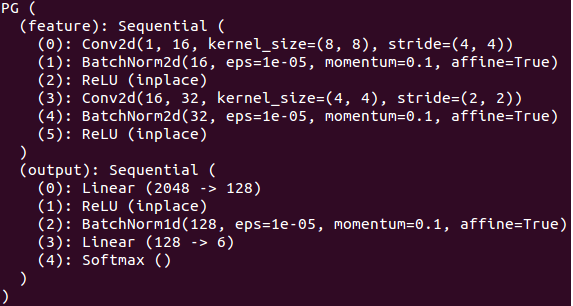
\includegraphics[scale=0.5]{pg_model_text.png}\label{fig:f1}}
\hfill
\subfloat[DQN model (text)]{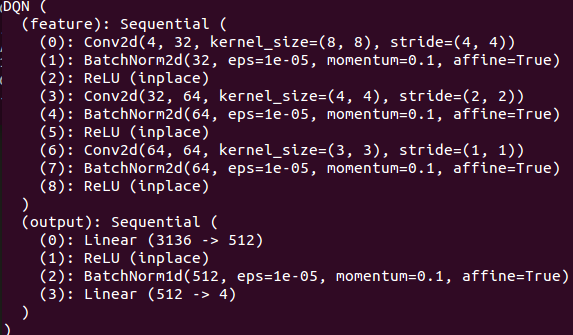
\includegraphics[scale=0.5]{dqn_model_text.png}\label{fig:f2}}
\hfill
\caption{Model structures}
\label{fig:f3}
\end{figure}

\begin{table}[!htb]
\centering
\begin{tabular}{|c|c|}
\hline
{\textbf{total episode}} & {\textbf{best test reward}}\\
\hline
{7000} & {9.03}\\
\hline
\hline
{\textbf{optimizer, learning rate}} & {\textbf{reward decay}} \\
\hline
{RMSprop, $10^{-3}$} & {0.99}\\
\hline

\end{tabular} 
\caption{PG model settings (best test reward是用得到最高的training reward的model算的)}
\label{table:1}
\end{table}

\begin{table}[!htb]
\centering
\begin{tabular}{|c|c|c|}
\hline
{\textbf{total episode}} & {\textbf{best test reward}} & \textbf{replay memory} \\
\hline
{40000} & {68.32} & {10000} \\
\hline
\hline
{\textbf{optimizer, learning rate}} & {\textbf{reward decay}} & \textbf{episodes before learning} \\
\hline
{RMSprop, $2.5 \times 10^{-4}$} & {0.99} & {1000 episodes}\\
\hline
\hline
\textbf{batch size} & \textbf{update freq. of target model} & \textbf{update freq. of online model}\\
\hline
{64} & {50 episodes} & {4 actions}\\
\hline

\end{tabular} 
\caption{DQN model settings (best test reward是用得到最高的training reward的model算的)}
\label{table:2}
\end{table}

\begin{figure}[!htb]
\centering
\subfloat[Pong (pg)]{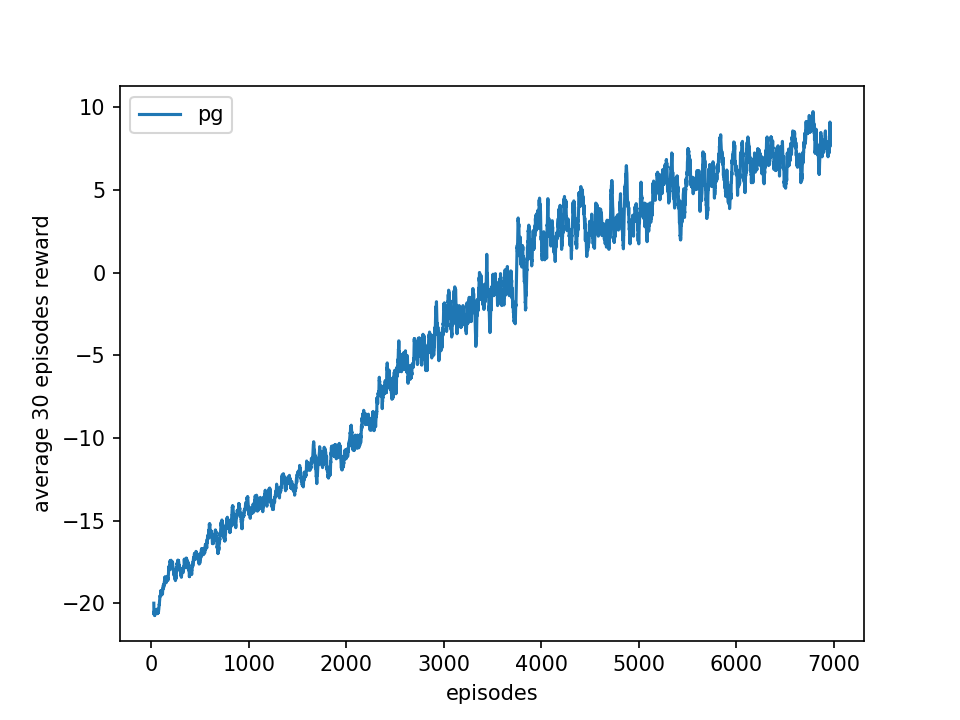
\includegraphics[scale=0.5]{pg_avg_reward.png}\label{fig:f4}}
\hfill
\subfloat[Breakout (DQN)]{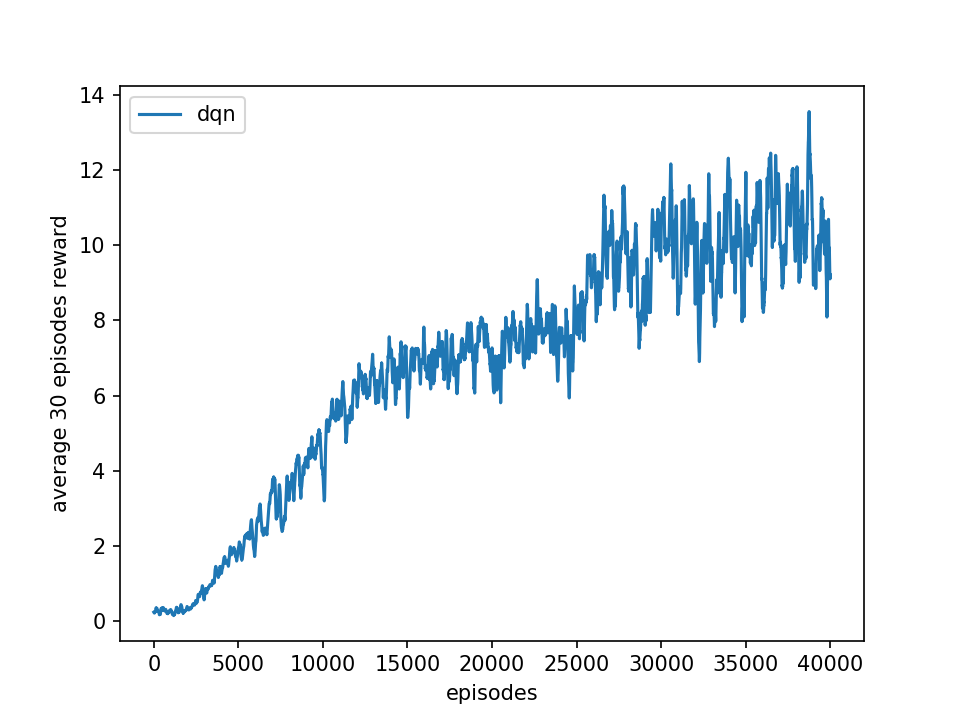
\includegraphics[scale=0.5]{dqn_avg_reward.png}\label{fig:f5}}
\hfill
\caption{Learning curves, average reward of last 30 episodes to numbers of episodes}
\label{fig:f6}
\end{figure}


\section{Experimenting with DQN hyperparameters}
我選擇的參數是replay memory,因為一開始在還沒使用助教公佈的參數時,我用10000的memory size時的training reward大概在3 $\sim$ 4分,但是同樣的場數用500000 memory size卻可以train到7 $\sim$ 8分,因此覺得memory size應該對model影響很大,所以選擇了他。\\
由Figure \ref{fig:f7}可以看出replay memory對於model的影響的確頗巨大的,基本上memory愈大的話reward幾乎都愈高,而且幾乎training從頭到尾都是領先的。因為memory size調大的話,可以記住較多前面幾場exploration後留下的結果,因此在training的時候也較容易sample到那些state(因為exploration主要在training前期,若是memory太小一下就被洗掉了),所以model等於是可以比較好explore到reward高的地方,進而讓training更好。\\
但是也可以發現memory size愈大的在training中後期的變動是較大的,因為在中後期大部份state可能都探索過了,在reward都趨於穩定的情況下,若是memory size較大的話就會記住那些用很久以前的Q function所進行的遊戲,但是那時候的Q肯定較差,導致那時候選擇的action可能有問題,因此若sample到那些點可能會讓Q function更新出錯。但是因為Q function本來就不是完美的,因此舊的Q function選擇的action可能誤打誤撞選到對的,因此這樣的出錯會導致結果有好有壞,因此learning curve變動較大。

\begin{figure}[!htb]
\centering
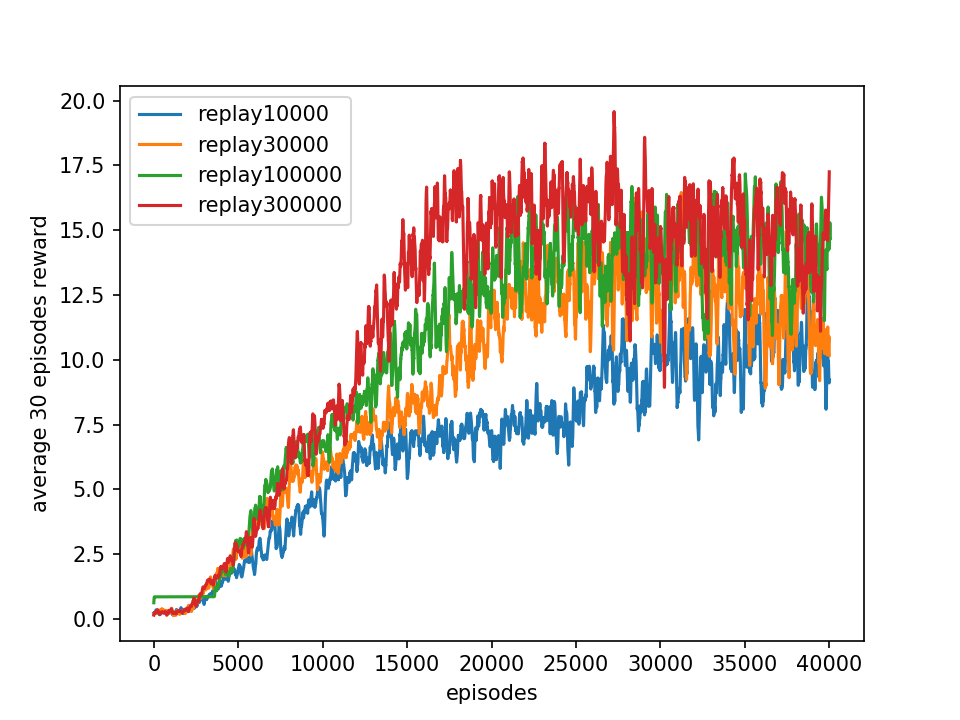
\includegraphics[scale=0.7]{replaysize_avg_reward.png}

\caption{DQN learning curve (different size of replay memory)}
\label{fig:f7}
\end{figure}



\section{Bonus}

\subsection{Improvements to DQN}
我實作的兩個DQN的improvement是double DQN以及dueling DQN。
\subsubsection{Double DQN}
Double DQN是用online model來選擇action,用target model來評估下一個state及action的好壞,如此用同一個model選擇action及評估會造成高估某一個action的問題可以被減小。Double DQN的目標函數如下:
\[ \mathbb{E}[(r + \gamma max_{a'}Q(s', argmax_{a'}Q(s',a',w), w^{-}) - Q(s, a, w))^2] \]
我利用double DQN玩breakout的結果如Figure \ref{fig:f8},基本上其餘參數設定都和原本的DQN一模一樣。我發現double DQN玩這個遊戲的結果在40000個episodes內是比原本的DQN差的,但是double DQN其實仍然在成長,只是為了和DQN比較就只能停在40000場遊戲了。有兩個可以觀察的地方,第一個是Double DQN成長速度較慢,第二個是Double DQN training變動比較小。第一個我認為是因為breakout這個遊戲主要只有左右移動兩個動作,因此用傳統的DQN學習greedy一點也不太容易出錯,而且這樣greedy的更新某個動作,若那個動作是好的就會學習較快。同時這也對應到第二個問題,太greedy的更新會導致若發現了另一個好的動作後,就會馬上更新成該動作,因此training的變化會比較劇烈。

\begin{figure}[!htb]
\centering
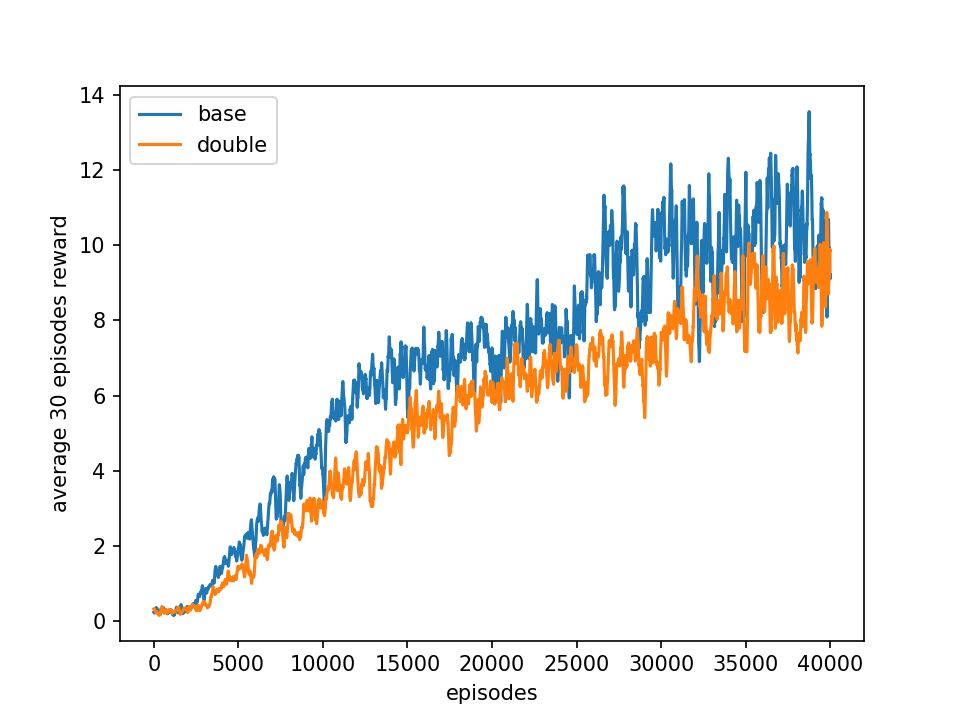
\includegraphics[scale=0.7]{dqn_db_avg_reward.png}

\caption{DQN learning curve (double DQN vs DQN)}
\label{fig:f8}
\end{figure}

\subsubsection{Dueling DQN}
Dueling DQN是將network的輸出$Q(s,a)$改成$V(s)+A(s,a)$,這樣一來network更可以分別學到每個state的以及搭配action後的分數如何。從Figure \ref{fig:f9} 可以發現dueling DQN表現確實比較好,因為他可以明確的學到state的分數以及action的分數,因此model可能會更偏向移動到state分數比較高的地方以獲取比較好reward。但是dueling DQN training的變化又更大了,我想是因為output有兩個network,要兩個network一起合作輸出就會造成變動是兩個network加起來的。
\begin{figure}[!htb]
\centering
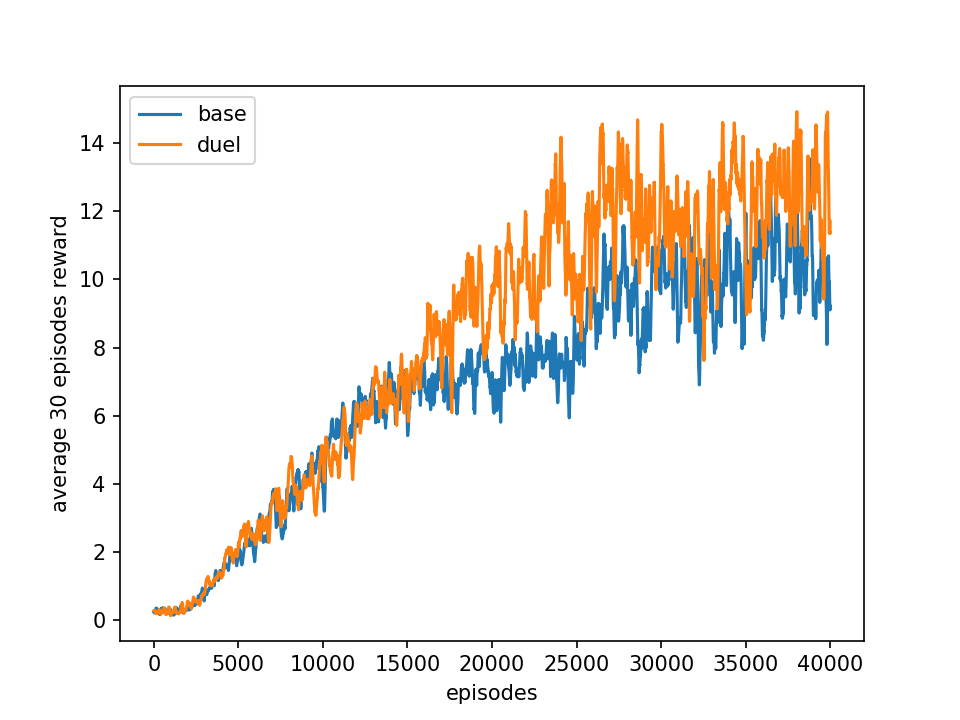
\includegraphics[scale=0.7]{dqn_duel_avg_reward.png}

\caption{DQN learning curve (dueling DQN vs DQN)}
\label{fig:f9}
\end{figure}


\subsection{Implement other advanced RL method, describe what it is and why it is better}

我實作的是Asynchronous Advantage Actor-Critic(A3C)演算法,他合併了policy gradient和Q learning兩個演算法的好處,訓練一個model可以output每個action被選擇的機率,以及可以output每個state的分數(該state未來的reward)。核心的概念是有一個actor學習如何選擇action來得到最高的reward,搭配一個critic判斷actor的表現如何,若是actor現在得到的reward大於critic給的,那麼就鼓勵actor做這個動作,reward較低則相反。而critic也會學習如何打分數更準(output更準的state分數)。因此兩個model的目標函數就可以如下表示:\\
Actor要maximize以下目標:
\[\mathcal{R}(\theta^{a})=\frac{1}{N}\sum_{n=1}^N\sum_{t=1}^{T_n}(R_n^t - V(s_t^n; \theta^{c}))log(p(a_t^n|s_t^n, \theta^{a})) \]
Critic要minimize以下目標:
\[L(\theta^c) = \frac{1}{N}\sum_{n=1}^N\sum_{t=1}^{T_n}(R_n^t - V(s_t^n; \theta^{c}))^2 \]
傳統的policy gradient只能玩完整場才知道策略的好壞,並且更新參數,這樣的作法缺點是variance太大。這個演算法相較於policy gradient的好處是可以訓練一個critic對每個state打分數,這樣就可以用Temporal-Difference(TD)的方式更新參數,但是這個state分數是這個state以後期望的reward,所以又有Monte-Carlo的性質,因此可以結合兩個方法的好處。而比DQN好的地方就是有actor可以自己決定該怎麼移動,而不是只是靠critic給的分數高低來移動。\\
而Asynchronous的意思是利用很多個agent在不同的environment setting下玩遊戲,因此學出來的model會遇過更多情況,表現也會更好。\\
最後是actor和critic的model可以共用參數,因為他們都是看影片學習怎麼移動(打分數),因此convolution layer的部份應該可以共用。(可參考Figure \ref{fig:f12})\\

\begin{figure}[!htb]
\centering
\subfloat[A3C model (https://medium.com/emergent-future/simple-reinforcement-learning-with-tensorflow-part-8-asynchronous-actor-critic-agents-a3c-c88f72a5e9f2)]{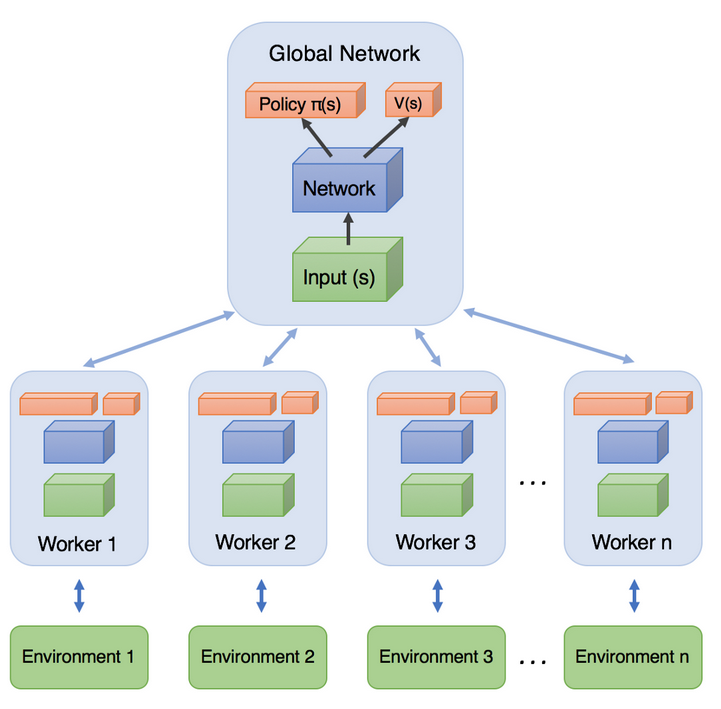
\includegraphics[scale=0.4]{a3c.png}\label{fig:f10}}
\hfill
\subfloat[Actor and Critic share part of the model (MLDS 12/7上課投影片)]{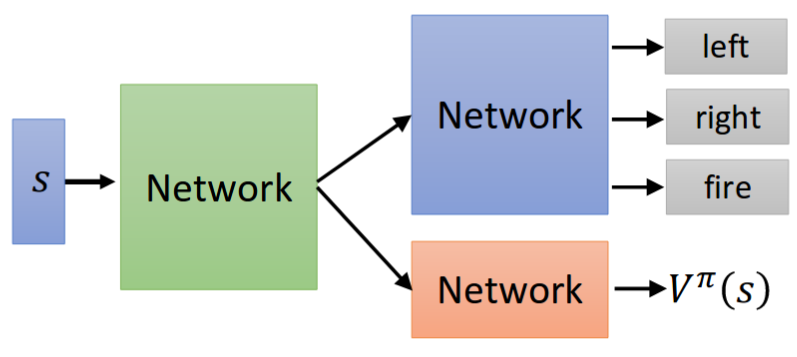
\includegraphics[scale=0.4]{share_model.png}\label{fig:f11}}
\hfill
\caption{Learning curves, average reward of last 30 episodes to numbers of episodes}
\label{fig:f12}
\end{figure}
\noindent
我A3C model的設定跟pg幾乎一樣,只是拿掉了batch normalization(加了結果差不多),並且用了16個actor來訓練,設定如Table \ref{table:3}所示。
Figure \ref{fig:f12} 是我把a3c玩在pong上面的結果,可以發現的確比傳統的pg還要好,玩到400多場遊戲就可以突破10分(只不過若把所有actor加起來的話就算玩6400場了...)。只不過learning curve 看起來有點崎嶇,我想應該是我learning rate調太大和因為有16個不同的actor在訓練導致variance較大的緣故。

\begin{table}[!htb]
\centering
\begin{tabular}{|c|c|}
\hline
{\textbf{total episode}} & {\textbf{num of actors}}\\
\hline
{425} & {16}\\
\hline
\hline
{\textbf{optimizer, learning rate}} & {\textbf{reward decay}} \\
\hline
{ADAM, $10^{-2}$} & {0.99}\\
\hline

\end{tabular} 
\caption{A3C model settings}
\label{table:3}
\end{table}

\begin{figure}[!htb]
\centering
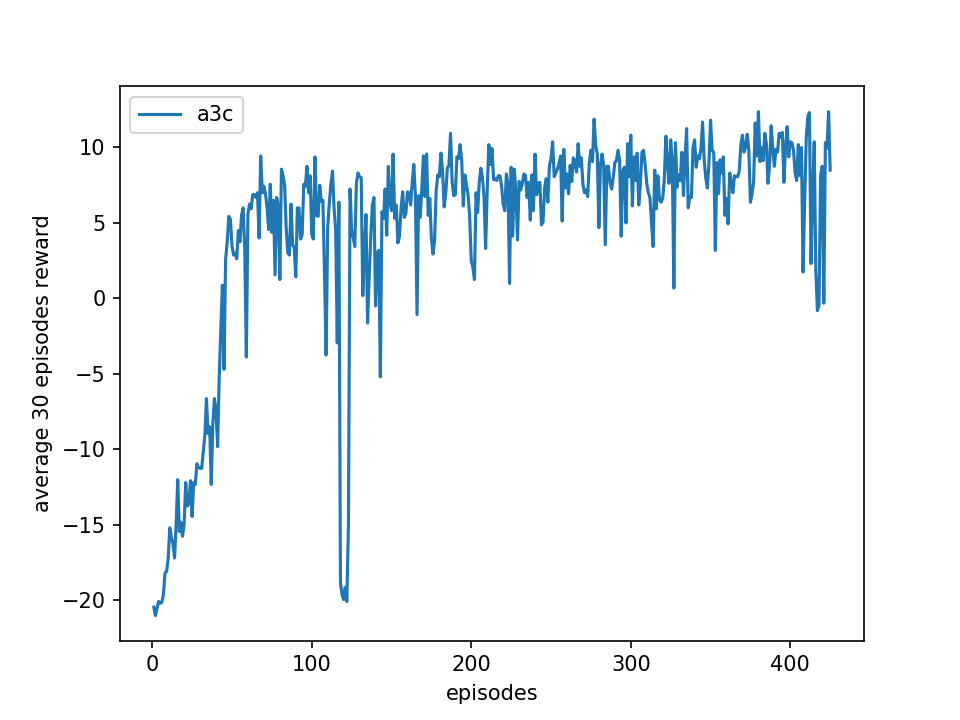
\includegraphics[scale=0.7]{a3c_avg_reward.png}
\caption{a3c learning curve (playing Pong)}
\label{fig:f11}
\end{figure}

\section{Reference}
\noindent

\url{https://www.zhihu.com/question/56692640}\par
\url{https://www.csie.ntu.edu.tw/~yvchen/f106-adl/doc/171204+171207_DeepRL2.pdf}\par
\url{https://medium.com/emergent-future/simple-reinforcement-learning-with-tensorflow-part-8-asynchronous-actor-critic-agents-a3c-c88f72a5e9f2}\par
\url{https://arxiv.org/pdf/1602.01783.pdf}\par
\url{https://gist.github.com/sangmin082/461079044a6686b7566319b4b7afad4a#new_comment_field}\par
\url{https://github.com/transedward/pytorch-dqn}\par
\url{http://pytorch.org/tutorials/intermediate/reinforcement_q_learning.html}\par
\end{CJK}

\end{document}
